%%%%%%%%%%%%%%%%%%%%%%%%%%%%%%%%%%%%%%%%%
% Uppsala University Assignment Title Page
% LaTeX Template
% Version 1.0 (27/12/12)
%
% This template has been downloaded from:
% http://www.LaTeXTemplates.com
%
% Original author:
% WikiBooks (http://en.wikibooks.org/wiki/LaTeX/Title_Creation)
% Modified by Elsa Slattegard to fit Uppsala university
% License:
% CC BY-NC-SA 3.0 (http://creativecommons.org/licenses/by-nc-sa/3.0/)

%\title{Title page with logo}
%----------------------------------------------------------------------------------------
%	PACKAGES AND OTHER DOCUMENT CONFIGURATIONS
%----------------------------------------------------------------------------------------

\documentclass[12pt]{article}
\usepackage[english]{babel}
\usepackage[utf8x]{inputenc}
\usepackage{amsmath}
\usepackage{graphicx}
\usepackage{float}
\usepackage[colorinlistoftodos]{todonotes}
\usepackage{pdfpages}

\setcounter{tocdepth}{1} % Show sections
%\setcounter{tocdepth}{2} % + subsections
%\setcounter{tocdepth}{3} % + subsubsections
%\setcounter{tocdepth}{4} % + paragraphs
%\setcounter{tocdepth}{5} % + subparagraphs
\renewcommand*\contentsname{Sumário}

\usepackage{hyperref}


\begin{document}

\begin{titlepage}

\newcommand{\HRule}{\rule{\linewidth}{0.5mm}} % Defines a new command for the horizontal lines, change thickness here

\center % Center everything on the page

%----------------------------------------------------------------------------------------
%	HEADING SECTIONS
%----------------------------------------------------------------------------------------

\textsc{\LARGE Universidade Paulista}\\[1.5cm] % Name of your university/college

\includegraphics[scale=.3]{unip.jpg}\\[1cm] % Include a department/university logo - this will require the graphicx package
\textsc{\Large Ciência da Computação}\\[0.5cm] % Major heading such as course name
\textsc{\large 1/2 semestre}\\[0.5cm] % Minor heading such as course title
\textsc{\Large Atividades Práticas Supervisionadas (APS)}\\[0.5cm] % Major heading such as course name
%----------------------------------------------------------------------------------------
%	TITLE SECTION
%----------------------------------------------------------------------------------------

\HRule \\[0.4cm]
{ \Large \bfseries Projeto de Reconhecimento de Letras no Alfabeto}\\[0.4cm] % Title of your document
\HRule \\[1.5cm]

%----------------------------------------------------------------------------------------
%	AUTHOR SECTION
%----------------------------------------------------------------------------------------

% \begin{minipage}{0.4\textwidth}
% \begin{flushleft} \large
% \emph{Author:}\\
% First name \textsc{Last name}\\ % Your name
% \end{flushleft}
%
% \end{minipage}\\[2cm]

% If you don't want a supervisor, uncomment the two lines below and remove the section above
%\Large \emph{Author:}\\
%John \textsc{Smith}\\[3cm] % Your name

%----------------------------------------------------------------------------------------
%	DATE SECTION
%----------------------------------------------------------------------------------------

{\large \today}\\[2cm] % Date, change the \today to a set date if you want to be precise

\vfill % Fill the rest of the page with whitespace

\end{titlepage}



\tableofcontents





* PROPOSTA DO TRABALHO
* APRESENTAÇÃO DO TRABALHO
ATIVIDADES PRÁTICAS SUPERVISIONADAS (APS)



II. PROPOSTA DO TRABALHO





III. Estrutura do Trabalho





IV. Ficha de Atividades Práticas Supervisionada
O trabalho deve ter obrigatoriamente uma ficha de atividades com entradas indicando quanto cada aluno trabalhou, a data que o trabalho foi feito, e qual atividade foi feita naquela data. Cada entrada deve obrigatoriamente ser assinada à mão pelo aluno.




V. MODELO DE FICHA DE ATIVIDADES PRÁTICAS SUPERVISIONADAS

\section{Estrutura do Trabalho}


O grupo pode usar qualquer estrutura que escolher. Mas é aconselhável que use a seguinte estrutura como roteiro:

\begin{description}
\item[Resumo]:
Resumo do trabalho, explicação do problema, quais foram as técnicas utilizadas, e quais foram os resultados
Tamanho ideal: 1/2 página. Tamanho máximo: 1 página
\end{description}


Introdução:
Explicação do problema, motivação e importância de resolver o problema, como que a solução pode ser aplicada no mundo real. Explicação do conjunto de dados, como que os dados foram coletados. Indicação de outros trabalhos que tentaram resolver o problema ou algum problema semelhante.
Tamanho ideal: 1 página e meia. Tamanho máximo: 3 páginas (sem contar imagens, se houver)


Referencial Teórico e Ferramentas:
Explicação da teoria e informação que o leitor precisa saber para conseguir ler o seu trabalho. Supondo que o leitor tenha conhecimento básico de um curso de Ciência da Computação.


Métodos:
Quais foram os métodos utilizados para resolver o problema. Como que a base de dados foi dividida. Qual foi o pré-processamento que foi aplicado na base de dados.


Resultados:
Quais foram os resultados que o seu trabalho obteve. Como foi feita a avaliação dos resultados.


Conclusão:
O que podemos concluir a partir dos resultados. Qual técnica teve uma melhor avaliação segundo qual critério.


Trabalhos Futuros:
Como que seu trabalho pode ser melhorado futuramente.


Referências Bibliográficas:
Lista do material consultado para fazer o trabalho.



\section{Proposta do Trabalho}

O grupo deverá fazer um estudo de técnicas de reconhecimento de imagens contendo letras do alfabeto escritas à mão. Para este trabalho será avaliado somente o reconhecimento da letra “i” maiúsculo e minúsculo, entre outras vogais do alfabeto. O objetivo do trabalho é fazer um programa que responda se uma imagem de uma letra vogal escrita à mão é a letra “i” ou não.


Será disponibilizado um conjunto de dados retirado da página https://www.nist.gov/srd/nist-special-database-19. O grupo deve usar apenas as letras vogais maiúsculo e minúsculo. É aconselhável que o grupo use apenas uma parte do conjunto de dados, visto que o conjunto todo é muito grande e pode fazer o treinamento demorar muito. Uma parte considerável do conjunto pode ser baixada no
% \href{https://viniciusdenovaes.github.io/aulas/unip/20222/pi_files/trabalhos/03/trabalho03.html}{site da APS}.


O grupo deverá aplicar técnicas de Aprendizado de Máquina para resolver o problema. De preferência deverão ser aplicadas mais de uma técnica diferentes para resolver o problema, que deverão ser avaliadas segundo os critérios de acurácia, precisão, recall, e pontuação f1.


As técnicas e avaliação de cada técnica deverão ser apresentadas no trabalho.


\section{Apresentação do Trabalho}

\renewcommand{\labelenumi}{\arabic{enumi}.}
\renewcommand{\labelenumii}{\arabic{enumi}.\arabic{enumii}.}
\renewcommand{\labelenumiii}{\arabic{enumi}.\arabic{enumii}.\arabic{enumiii}.}
\begin{enumerate}
\item O grupo deverá ser composto de 5 alunos. A formação de um grupo com um
número diferente de 5 dependerá de aprovação do(a) Coordenador(a) Auxiliar do
curso no campus.
\item Todas as etapas do trabalho deverão ser escritas em fonte ARIAL 12,
espaçamento 1,5, margem direita 2,5 cm e margem esquerda 2,5 cm. O trabalho
deverá ter formato A4, encadernado (espiral) com capa transparente.
\item Limites de páginas
\begin{itemize}
\item Objetivo do trabalho: 1 página e no máximo 2 páginas
\item Introdução: 2 páginas e no máximo 4 páginas
\item Criptografia (conceitos gerais): 3 páginas e no máximo 5 páginas.
\item Técnicas criptográficas mais utilizadas: mínimo de 4 páginas e máximo de 8
páginas.
\item Dissertação: mínimo de 5 páginas e máximo de 15 páginas.
\item Projeto (estrutura) do programa: mínimo de 3 páginas e máximo de 8 páginas.
\item Relatório com as linhas de código: máximo de 10 páginas.
\end{itemize}
\item O trabalho deverá ser entregue junto no site com a ficha padrão de “Atividades Práticas
Supervisionadas” ilustrando cronologicamente cada um dos itens, segundo a
orientação do professor supervisor desta atividade.
\item Estrutura do trabalho:

\begin{enumerate}

\item Capa: identificando o curso, o tema, a relação de alunos do grupo (nome/RA)
\item Índice
\item Objetivo do trabalho
\item Introdução
\item Criptografia (conceitos gerais)
\item Técnicas criptográficas mais utilizadas e conhecidas
\item Dissertação (*** Sua técnica criptográfica escolhida***)
\begin{enumerate}

\item Estruturação, conceitos e fundamentação
\item Benefícios em relação às técnicas anteriores.
\item Aplicações que fazem/fizeram uso da técnica.
\item Discussão comparativa entre esta técnica e outras conhecidas /
utilizadas
\item Vulnerabilidades e falhas.
\item Melhorias propostas e/ou implementadas.

\end{enumerate}
\item Projeto (estrutura) do programa
\item Relatório com as linhas de código do programa
\item Apresentação do programa em funcionamento em um computador,
apresentando todas as funcionalidades pedidas e extras.
\item Bibliografia
\item Ficha de Atividades Práticas Supervisionadas
\end{enumerate}

\end{enumerate}

\section{Modelo de Ficha de Atividades Práticas Supervisionadas}
Na página seguinte em anexo



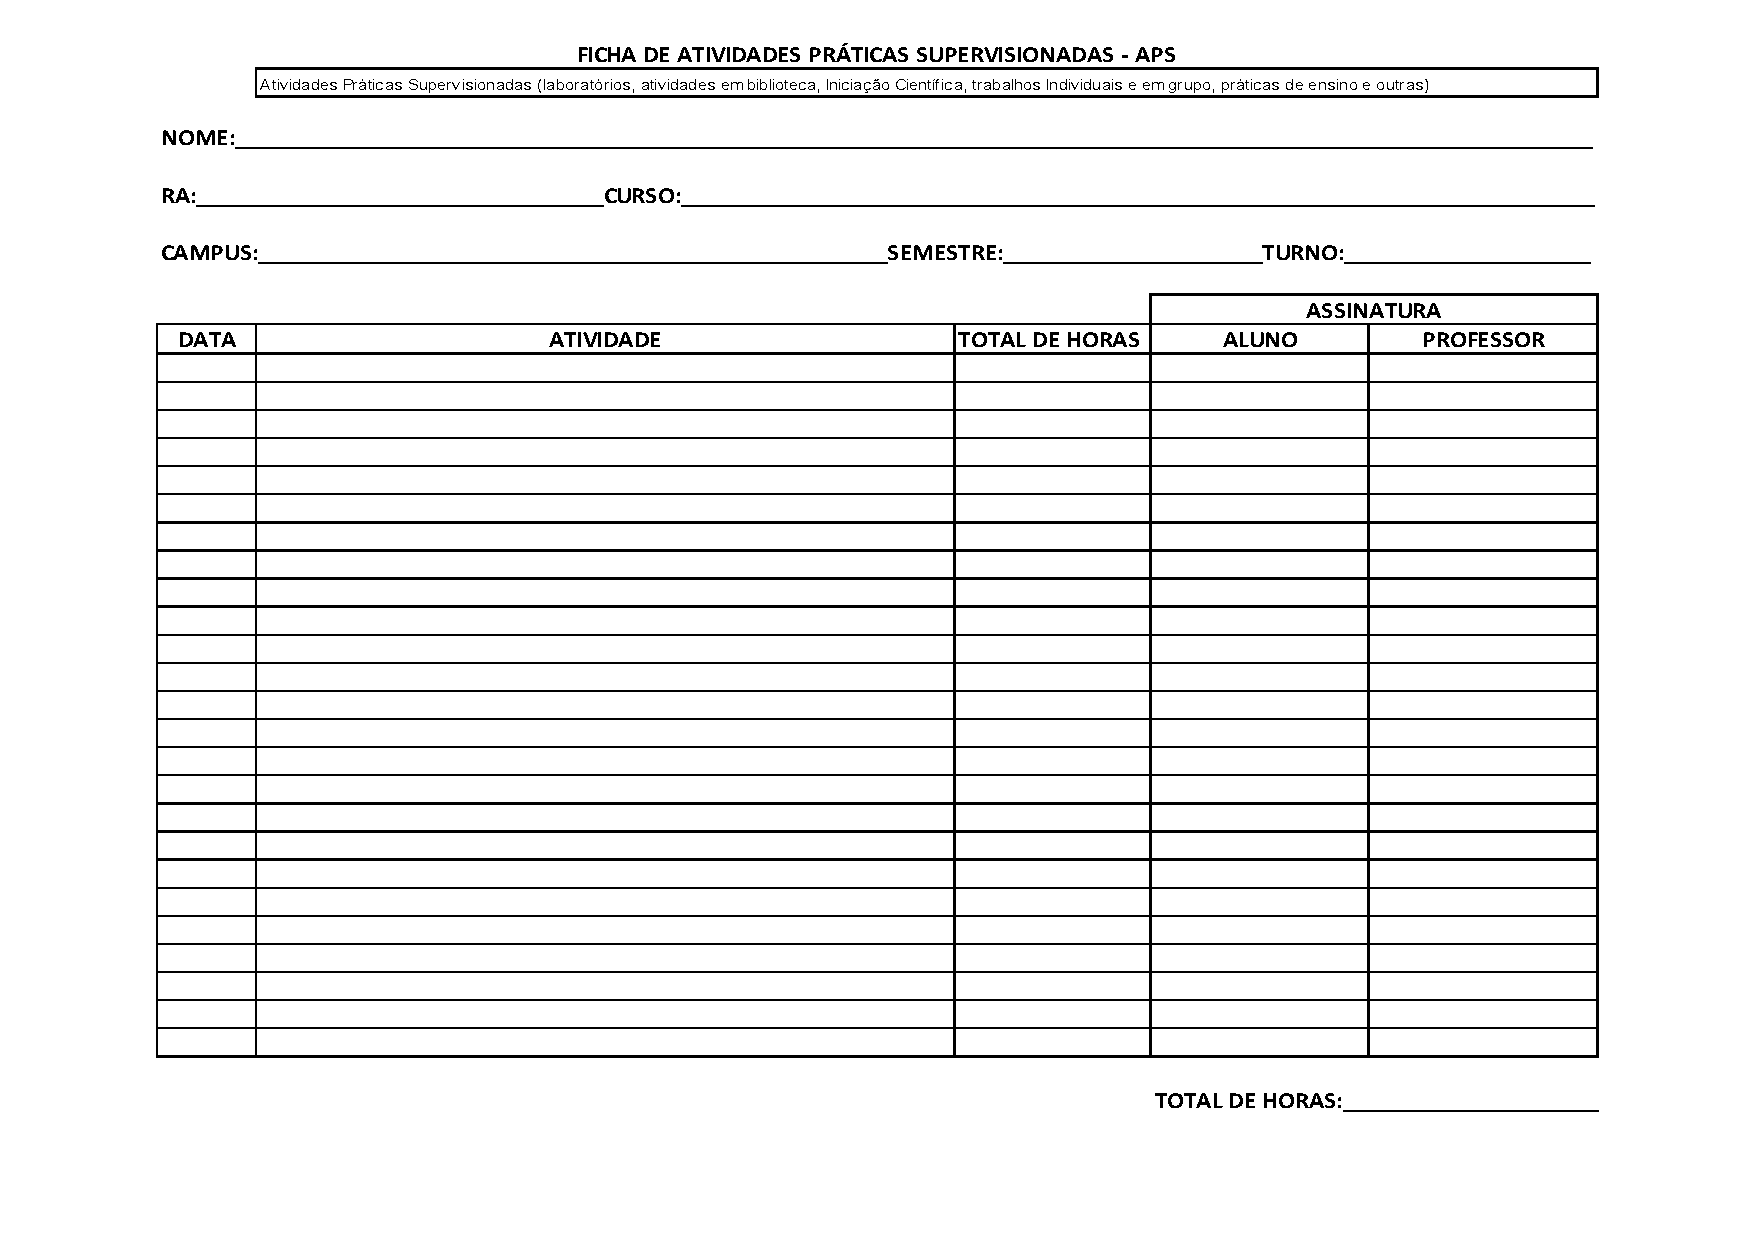
\includepdf[landscape=true]{ficha_atividades.pdf}




















\end{document}
